\section{Analysis techniques}

In this work, the structure factor derived domain size, geometric pore size distribution and tortuosity will be 
utilized to characterize the microstructure. The nematic order parameter will be used to characterize the particle 
order to the magnetic field. The average angle to the interface will be utilized to characterize how the particles 
ordering to the field affect the interface position. Finally, the radial distribution function will be used to probe 
how differences in ordering change the packing of particles on the interface. The time evolution of viscosity will 
provide insight into the rheological properties of the bijel, while the aforementioned analysis tools in addition to 
proportion of particles on the interface will be calculated to provide insight into how the bijel reacts to shear, 
parallel and perpendicular to the magnetic field. A more detailed description of the implementation of each method is 
shown in subsequent sections.

\subsection{Particle filling and interface smoothening}
\label{section:filling_routine}

Particles are the cause of bijels but they can also make characterization of domain size, curvature, pore size 
distribution and tortuosity more difficult as particles may change these parameters. An extrapolation scheme is 
required to connect the interface one different sides of the particles and to fill in the particles themselves so 
as to create a more accurate interface for other techniques.

This is accomplished through sequential density averaging and filling of grid points making up the particles from 
the outside in. The grid cells around a cell of interest are averaged using a D3Q19 like lattice and stepping through 
all points with a order parameter $\phi = \rho^w - \rho^o$ value of 0. 

\subsection{Domain size}
\label{section:domain_size}

The characteristic length scale at time $t$ of a bijel can be computed from the moments of the structure factor. The 
structure factor is first calculated from the order parameter of the phases, defined as $\phi = \rho_b - \rho_r$ where 
$\phi$ is the density order parameter and $\rho_b$ and $\rho_r$ are the densities of the blue and red fluid respectively. 
Next, the fluctuations of the order parameter $\phi'$ is calculated by subtracting the mean of the order parameter, 
$\langle \phi \rangle$ from the order parameter, defined as $\phi' = \phi - \langle \phi \rangle$. Next, the fourier 
transform of the fluctuations of the order parameter $\phi'(\mathbf{k})$ is calculated. Finally, $\phi'(\mathbf{k})$ 
is squared and made positive and normalized by the volume of the system defined as 
$S(\mathbf{k}) = \frac{1}{N} |\phi'(\mathbf{k})^2|$.

The first domain size metric used is the domain size derived from the spherically averaged first moment of the structure 
factor. The spherical averaging is done by averaging the values of the structure factor at the same $\mathbf{k}$ up 
till the nyquist frequency. The spherically averaged structure factor is defined as $S(k)$ where $k$ represents the 
wave numbers obtained from the spherical averaging. Next, the first moment $\langle k_1 \rangle$ is calculated as 
$\langle k_1 \rangle = \frac{\Sigma_{k} k\cdot S(k)}{\Sigma_{k} S(k)}$. Finally, the domain size is calculated as 
$L_1 = \frac{2 \pi}{\langle k_1 \rangle}$. \cite{kendon_inertial_2001,kendon_3d_1999} This domain size is used in past literature 
to calculate the correct scaling regime of a system undergoing spinodal decomposition. 

While it cannot be used to correlate physical phenomena the second moment of the structure factor derived domain 
size is utilized here to discriminate directional length scales. Owing to the spherical averaging done, the first 
moment moment derived domain size is unable to be used to calculate direction specific length scales. The second 
moment of the structure factor is first calculated by multiplying 
$\langle \mathbf{k_2}^2 \rangle = \frac{\Sigma_{\mathbf{k}} \mathbf{k}^2 S(\mathbf{k})}{\Sigma_k S(\mathbf{k})}$ 
where $\mathbf{k_2}^2$ represents the second moment in each cartesian direction. Next, the domain size in each 
direction is calculated as $L_2 = \frac{2 \pi}{\sqrt{\mathbf{k_2}^2}}$. \cite{jansen_bijels_2011, gunther_timescales_2014} 
In the rest of this document, $L_{\parallel}$ and $L_{\perp}$ is defined as the domain size parallel and perpendicular to 
the applied magnetic field.

\subsection{Curvature}
\label{section:curvature}

The simulation data was first pre-processed by calculating the order parameter of the densities, defined as the difference between the blue and red 
fluid densities at each grid point. $\phi(\vec{x}) = \rho^b(\vec{x}) - \rho^r(\vec{x})$. We then apply the particle filling algorithm described in 
section \ref{section:filling_routine} to the $\phi$ distribution, This reduces error from the presence of particles at the interface, 
resulting in an interface geometry that is more accurate to the bijel interface profile. From the filled order parameter, $\phi$, we calculate the mesh of 
the iso-surface representing the interface at $\phi = 0$ using a marching cubes method as implemented in scikit-image. We then use pyvista to calculate the 
gaussian and mean curvatures of the bijel microstructure, in addition to the interface area. The radii of curvature, $R_1, R_2$ are calculated from the 
mesh through measuring the angles between nearest neighbors and the laplacian of the faces to calculate the Gaussian and mean curvature respectively. 

We then limit the values of the calculated Gaussian and mean curvatures to reduce the effect of numerical artefacts created during the meshing process. We 
limit the Gaussian and mean curvatures to the expected curvatures around $|H| \approx \frac{2}{L}$ and $|K| \approx (\frac{2}{L})^2$. $L$ here is defined 
as the characteristic length scale obtained from the first moment of the spherically averaged structure factor described in section \ref{section:domain_size}.  
We then calculate an interface area normalized curvatures to remove the differences in absolute curvature values arising from the change in the characteristic 
length scale by calculating the surface area to volume ratio, $\Sigma = A_{int}/V$ where $A_{int}$ is the interfacial area and $V$ is the system volume. After 
dividing the obtained curvatures with $Sigma$, we obtain the discrete quantities, $H \Sigma^{-1}$ and $K \Sigma^{-2}$. For data presented as a time or magnetic 
field series, we sum each curvature distributions yielding, $\langle H \Sigma^{-1} \rangle$ and $\langle K \Sigma^{-2} \rangle$. For a bijel with volume ratio 
$50:50$ as used here, we expect $\langle K \Sigma^{-2} \rangle < 0$ and $\langle H \Sigma^{-1} \rangle \approx 0$.

\subsection{Tortuosity}
\label{section:tortuosity}

Tortuosity can be defined as the ratio between the path length $(L_{eff})$ of two points and the euclidean distance 
between two points $L_{0}$, $\tau = L_{eff}/L_{0}$. In practice this is the geometric definition of tortuosity as 
often the tortuosity of a system is dependent upon other factors. Diffusive tortuosity is what we will use here, 
defined as $\tau = \frac{D_{eff}}{D_0}$. This metric is also more relevant to the potential applications of bijels 
which rely on diffusion of mass for their uses.

Simulation techniques such as Lattice Boltzmann or Molecular Dynamics have been used to characterize the tortuosity of 
porous materials. However, these simulations can be computationally expensive and time consuming to perform, even though 
they may have great accuracy. Recently, particle diffusion techniques based on a random walk such as pytrax and taufactor 
or Pore Network Modelling (PNM) based techniques such as PoreSpy have been introduced which offer a tradeoff of accuracy 
for speed. Taufactor in particular is implemented on GPU's with a periodic boundary condition, allowing for rapid and 
accurate calculation of the tortuosity.

% \textcolor{blue}{https://joss.theoj.org/papers/10.21105/joss.05358, https://doi.org/10.1016/j.softx.2019.100277, https://joss.theoj.org/papers/10.21105/joss.01296}

Before using taufactor, the microstructure is first binarized. This is done by first calculating the order parameter of 
the system with $\phi = \rho_b - \rho_r$ where $\phi$ is the order parameter and $\rho_b, \rho_r$ are the densities of 
the blue and red fluid respectively. Next, the interface described with $\phi$ is smoothened using the algorithm detailed 
in section \ref{section:filling_routine}. \texttt{taufactor} determines the tortuosity by comparison
of steady-state diffusive flow through a porous medium with the bulk
diffusive flow in a control volume of the same size, molecular
diffusivity, and driving force \cite{cooper_taufactor_2016, kench_taufactor_2023}. We used
the \texttt{PeriodicSolver} to employ periodic boundary conditions. In many of the bijels synthesized using small molecule liquids, monomer is 
introduced into the oil phase and polymerized. Therefore, to perform the binarization step, we select all points where 
$\phi \leq 0$ and set their value to $0$, and all other values are set to $1$. To taufactor, $1$ represents void spaces 
and 0's are solid. \cite{cooper_taufactor_2016, kench_taufactor_2023}

\subsection{Interface order}
\label{section:interface_order}

We can calculate the ordering of the interface from the iso-surface of the interface. The simulation data was first pre-processed by calculating the 
order parameter of the densities, $\phi$. We then apply the particle filling algorithm described in section \ref{section:filling_routine} 
to the $\phi$ distribution. We then mesh the filled order parameter at $\phi = 0$ using the marching cubes algorithm and obtain the normals of the
vertices representing the points of the interface. We then computed the interfacial orientation tensor and plot that 
%
\begin{equation}
\tens{Q}_{\text{int}} = \frac{1}{\langle \mathrm{tr}(\tens{A}) \rangle} 
\left\langle \tens{A} - \frac{1}{3} \mathrm{tr}(\tens{A}) \mathsf{1} \right\rangle ,
\end{equation}
%
where the local tensor field $\tens{A}$ is defined by
%
\begin{equation}
\tens{A} = \nabla\phi\otimes\nabla\phi .
\end{equation}
%
The largest eigenvalue of $\tens{Q}$ is taken as the
interface nematic order parameter $S_{\text{int}}$.

\subsection{Channel size distribution}
\label{section:channel_size_distribution}

We use a method based on that outlined in Chan and Thornton. We create our distance function by performing an Eulerian Distance Transform on 
our order parameter data $\phi$ to obtain $\phi_{edt}$. \cite{chan_channel_2012} We smooth $\phi_{edt}$ using a boxcar algorithm with side length 3. 
We then normalize the distance from the interface in $\phi_{edt}$ using the characteristic length scale of the system defined as $\Sigma = \frac{V}{A_{int}}$
to obtain $\bar{\phi}_{edt}$ and a normalized distance from the interface, $\bar{r}$. A schematic of this workflow is demonstrated in Figure \ref{fig:csd_prep_viz}.

\begin{figure}
    \centering
    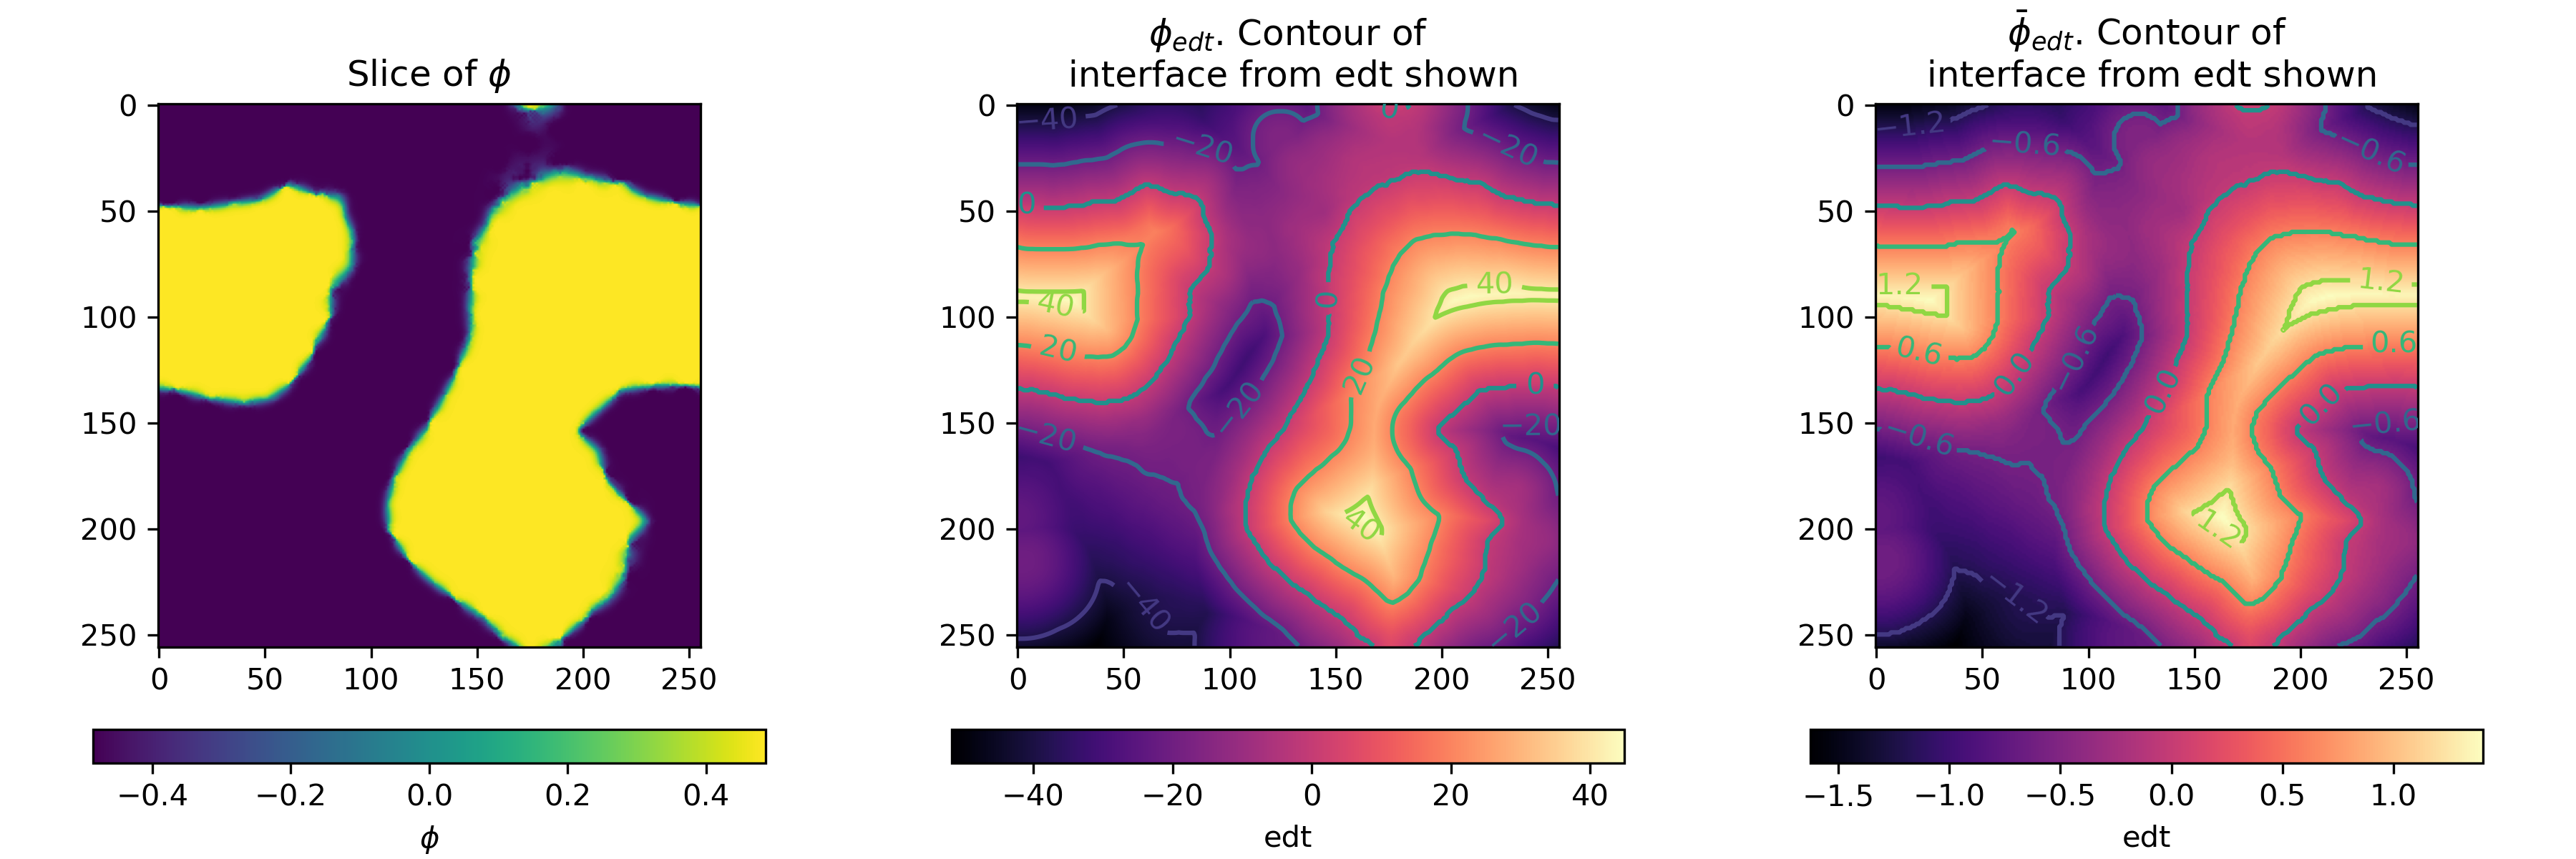
\includegraphics[scale = 0.4]{figures/analysis/csd_prep.png}
    \caption{Schematics detailing the order of operations of the steps to calculate the channel size distribution.}
    \label{fig:csd_prep_viz}
\end{figure}

The number of handles, $h$
in the iso-surface at different distances from the interface of $\bar{\phi}_{edt}$ is calculated. $h$ is also normalized by $\Sigma$ and the system volume
to obtain $\bar{h} = \frac{h}{V\Sigma^{-3}}$. The magnitude of the derivative of $\bar{h}$ with respect to $\bar{r}$, $f$, represents the channel size distribution.
A mean channel size can also be calculated from the first moment of the $f$.

\subsection{Nematic order parameter}
\label{section:nematic_order_parameter}

The orientational ordering of the particles to one another can be characterized using the nematic order parameter, 
defined as $S$. This parameter was first used to characterize liquid crystals. However its use has expanded to colloidal 
systems to characterize the ordering of a system to an average orientation, termed the director. A system is said to have 
nematic ordering if its components have orientational order to the director but does not require the system to have 
translational order.

The nematic order parameter is calculated from the orientational alignment tensor, $Q$, which is calculated from the 
orientation of particles to one another as 
$\langle Q \rangle = \frac{1}{N} \sum_{i}^{N} \langle \frac{3}{2}u_i u_i - \frac{1}{2}I \rangle$. $u_i$ is the 
orientation of particle $i$ and $I$ is an identity matrix. \cite{veerman_phase_1992} While there are multiple 
methods to evaluate the nematic order parameter, the one we have picked is where the largest eigenvector is $S$, 
with its corresponding eignvector referring to the director of the system. \cite{veerman_phase_1992} 
% \textcolor{blue}{https://doi.org/10.1080/00268978400101951} 
A system is defined to be ordered nematically, 
if $S > 0.3$. In this work, the direction of the director will be compared to the direction of the magnetic 
field. We utilize the implementation in Freud to calculate the nematic order parameter.

\subsection{Radial distribution function}
\label{section:radial_distribution}

The radial distribution function (RDF) is used to measure the normalized number density of particles around a 
reference particle as a function of distance. The normalization factor is the expected density of particles derived 
from an ideal gas. The general form of the equation to calculate the RDF is 
$g(r) = \frac{1}{\rho_{ideal}(r) 4\pi r^2} \int_{r}^{r+\Delta r} \delta(r_{i} - r_{j}) dr$ where $\rho_{ideal}(r)$ 
represents the density expected at distance r from a reference particle in an ideal gas, $\delta(r_{i} - r_{j})$ 
represents the number of particles within the bin $r + \Delta r$ and integrated to get a volumetric density. 
As implemented in a numerical method, the integral becomes a sum. After correcting for the periodic boundary 
condition using the minimum image convention, the RDF can be used to characterize periodic systems. We utilize 
the implementation in the software package Freud. \cite{ramasubramani_freud_2020}

\begin{equation}
    g(r) = \frac{n_p-1}{n_p} V \left\langle\delta\left(r-r_i\right)\right\rangle ,
\end{equation}

where \(n_p\) is the number of particles in the volume
\(V\), and \(\langle\cdot\rangle\) denotes an average over all
particles. The radial distribution function was calculated by binning
the distance between all particle pairs and normalizing the shells with
respect to the distribution \(4\pi \rho r^2 \mathrm{d}r\) of an ideal
gas. 

\subsection{Average interface angle and proportion of particles on the interface}
\label{section:interface_angle}

One way to differentiate between whether the particles pull the interface or whether the tilt of the particles at 
the interface causes changes to the jamming point is to characterize the average interface angle. The average interface 
angle $(\psi)$ is defined as the angle between the orientation of the axis of symmetry of the particle and the interface 
normal. The former mechanism would show little to no change in the interface angle, while the former mechanism should 
show large differences. The proportion of particles on the interface can also be calculated using this technique. 

The orientation of the particle is obtained from the output files from the simulation. The interface normal needs to 
be calculated from $\phi$. This is done by taking $\phi$ as calaculated from the red and blue fluid densities, then 
performing the particle fill routine described in section \ref{section:filling_routine}. Next, a mesh corresponding 
to the interface is obtained using a marching cubes algorithm at a countour level of 0 with a cube length of 4 lattice 
units, which corresponds to the thickness of the interface. \cite{van_der_walt_scikit-image:_2014} The 
position of the particle and its closest vertex is calculated. If this distance is larger than the first minimum in 
the radial distribution function, it is considered to be not on the interface and the next step is not performed. The 
vertex and corresponding normal closest to the position of a particle is used in the dot product, 
$\cos{\psi} = \frac{n_{int} \cdot o_{i}}{|n_{int}| |o_i|}$ where $n_{int}$ is the normal of the interface and $o_i$ 
is the orientation of particle i. After looping through all the particles, the average of $\psi$ and the number of 
particles in the interface is calculated.

\subsection{Steinhardt order parameter}
\label{section:steinhardt_order_parameter}

Another factor affected by the application of the magnetic field is the Steinhardt 6 fold order parameter, $Q6$, which characterized the local 
particle ordering. \cite{steinhardt_bond-orientational_1983} It has been used to characterize crystallization, glass transitions and crystal 
structures for colloidal and molecular crystals. We utilize the average across all particles on the interface, $\langle Q6 \rangle$ and track 
this parameter as a function of time. Past work has identified that local crystallization of colloidal crystals takes place at $\langle Q6 \rangle = 0.38$, 
and that $\langle Q6 \rangle^{HCP} = 0.485$. \cite{steinhardt_bond-orientational_1983, toxvaerd_role_2020, mickel_shortcomings_2013} We utilize a voronoi 
cell derived definition of the neighbor list of each particle, addressing some of the shortcomings highlighted in the original distance based definition. 
\cite{steinhardt_bond-orientational_1983, mickel_shortcomings_2013}. We first define a complex orientational vector, $q_{lm}$

\begin{equation}
q_{lm}(i) = \frac{1}{N_b(i)} \Sigma_{j = 1}^{N_b(i)} Y_{lm}(\vec{R}_{ij})
\end{equation}

Where $N_b$ is the number of nearest neighbors of particle $i$, $l$ is controls to the degree of spherical harmonic to be calculated, $m$ is an integer 
defined as $-l \leq m \leq l$ that defines which spherical harmonic is being calculated and $\vec{r}_{ij}$ is the distance between two particle centers. 
The neighbor list $N_b$ is usually defined by a cutoff distance from the center of particle $i$ to its nearest neighbors $j$. Steinhardt then defined a 
bond order parameter $q_l$ from $q_{lm}$ as

\begin{equation}
Q_{l}(i) = \sqrt{\frac{4 \pi}{2l + 1} \Sigma_{m = -l}^{l} |q_{lm}(i)|^2}
\end{equation}

In the literature, crystal structures can be distinguished from one another by plotting the distribution of two or more $Q_{l}$. 
\cite{lechner_accurate_2008, mickel_shortcomings_2013} Given that bijels form colloidal glasses, we only expect there to be
short range order which means conclusions made from this parameter can only be used to guide trends of order, not quantitative 
calculations of crystal structures.


\subsection{Shear stress}
\label{section:shear_viscosity}

In an incompressible fluid, the viscosity $(\eta)$ is defined as the ratio between the measured 
shear stress $(\sigma)$ and the applied strain rate $(\dot{\gamma})$, $\sigma = \eta \dot{\gamma}$. In rheological 
experiments, the viscosity is measured through a viscometer based on Couette or shear viscometry and Poiselle or 
pressure gradient viscometry. A Couette cell functions by applying a shear velocity to one or more walls, and measuring 
the shear stress response of the fluid. Common geometries for Couette cells include the cone and plate and concentric 
cylinder viscometers. In simulations, shear can be applied to walls of the simulation domain through either a shearing 
wall boundary condition or a Lees Edwards boundary condition. We select the Lees Edwards boundary condition as shearing 
results are unaffected by finite size effects and wall effects. Finite size effects are observed as a system size
dependent shear stress at the same shear rate. Wall effects can be seen as stick-slip effects of the particles or 
unphysical velocity gradients near the wall.

In a lattice boltzmann, the shear stress is measured as the sum of the equilibrium and nonequilibrium contributions.
\cite{kruger_shear_2009} These terms are defined as,

\begin{equation}
    \sigma_{\alpha \beta} = \sigma_{\alpha \beta}^{0} + \sigma_{\alpha \beta}^{1}
\end{equation}

This expression is obtained from the Chapman Enskog expansion of the lattice boltzmann method. The equilibrium and
non-equilibrium contributions of the stress are defined as

\begin{equation}
    \begin{split}
        \sigma_{\alpha \beta}^{0} &= \rho c_s^2 \delta_{\alpha \beta} + \rho u_{\alpha} u_{\beta} \\
        \sigma_{\alpha \beta}^{1} &= (1 - \frac{1}{2 \tau})\Sigma_{i} (f_{i} - f_{i}^{eq})c_{i \alpha}c_{i \beta} \\
    \end{split}
\end{equation}

In this work, a shear velocity is imparted in the z direction, across the x-axis. Therefore, the shear stress in the x 
and z directions, $\sigma_{xz}$, is measured. $\sigma_{xz}$ is output as calculated from the simulation for the entire 
domain after applying this equation to the system. 

% \subsection{Yield stress and zero shear rate viscosity}
% \label{section:yield_stress}

% The yield stress of bijels can be calculated using the flow curve, stress ramp or from oscillatory rheological techniques. 
% The flow curve method involves the steady application of shear, followed by measurements of the shear stress response of 
% the material. The plateau of the shear stress response is indicative of the steady state stress of the material. The stress ramp 
% method involves the application of a shear stress onto the material, followed by measurements of the strain rate. A 
% perfectly elastic material will have no strain rate, while a perfectly dissipative material will have high strain rate. 
% The yield stress is characterized as the point when a rapid increase in strain rate is observed. The yield stress from 
% oscillatory rheology is defined when the storage modulus is lower than the loss modulus. This work will utilize the flow 
% curve method.

% The shear viscosity calculated using the method detailed in Section \ref{section:shear_stress} will be plotted as a 
% function of applied shear rate. Rheological models such as the Herschel Buckley, Bingham Plastic or Carreu models can be 
% utilized to fit the shear viscosity as a function of shear rate to calculate the zero shear rate viscosity. In bijel 
% applications, this parameter gives insight into the material stability and processability.


% \subsection{Shear banding}
% \label{section:shear_banding}

% \textcolor{blue}{https://doi.org/10.1073/pnas.0812519106}

% \textcolor{blue}{https://doi.org/10.1103/PhysRevX.11.021017}